\section*{Q4: \texttt{grafico.py}}

Escreva um script para plotar as funções
%$$
%f_1(x)=\left\{
%\begin{aligned}
%x^2 \ \ \ \  \  \ \ \ \ \ &, 0\leq x < 4 \\
%16 \ \ \ \ \ \ \ \ \ \ \ &, 4\leq x < 6 \\
%(x-10)^2 \ \ \ \ \ \ \ \ \ \ \ &, 6\leq x < 10 \\
%-(x-10)^2 \ \ \ \ \ \ \ \ \ \ \ &, 10\leq x < 14 \\
%-16 \ \ \ \ \ \ \ \ \ \ \ &, 14\leq x < 16 \\
%-(x-20)^2 \ \ \ \ \ \ \ \ \ \ \ &, 16 \leq x < 20 \\
%\end{aligned}
%\right.
%$$

$$
g(x)=\left\{
\begin{aligned}
\dfrac{-1}{1+e^{6\cdot(x-1)}}+1 \  \ \ \ \ &, 0\leq x < 5 \\
\dfrac{-1}{1+e^{6\cdot(9-x)}}+1 \  \ \ \ \ &, 5\leq x < 10 \\
\dfrac{-1}{1+e^{6\cdot(11-x)}} \  \ \ \ \ &, 10\leq x < 15 \\
\dfrac{-1}{1+e^{6\cdot(x-19)}} \  \ \ \ \ &, 15\leq x < 20 \\
\end{aligned}
\right.
$$
e
$$
f(x)=\dfrac{\sqrt{6}}{2} \sin\left( \dfrac{\pi}{10}x\right)
$$
para o intervalo $0\leq x\leq 20$.

Além de plotar as duas funções sobrepostas, o script deve ainda adicionar grade, identificação dos eixos e legendas (replicar a figura abaixo).
\begin{figure}[htbp]
	\centering
		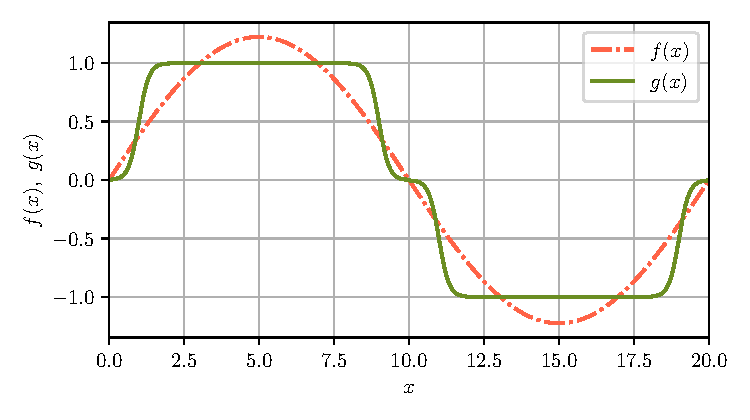
\includegraphics[scale=0.75]{figs/q4}
\end{figure}

